% Instituto Tecnologico de Costa Rica
% Maestría en Ciencias de la Computación
% Introducción a la Investigación
% II Semestre 2018
% 
% Author: Kathy Brenes Guerrero. 
% Profesor: Francisco Torres Rojas. 
% Chapter 3: Review of the Related Literature
%

\documentclass{beamer}
\usepackage{multicol}
\usepackage{csquotes}
\usepackage[pages=some]{background}

\backgroundsetup{
scale=1,
color=black,
opacity=0.4,
angle=0,
contents={%
  \includegraphics[width=\paperwidth,height=\paperheight]{figures/trafficJam}
  }%
}

\setbeamertemplate{navigation symbols}{}

\usetheme{Warsaw}

\newcounter{sauvegardeenumi}
\newcommand{\asuivre}{\setcounter{sauvegardeenumi}{\theenumi}}
\newcommand{\suite}{\setcounter{enumi}{\thesauvegardeenumi}}


\beamersetuncovermixins{\opaqueness<1>{25}}{\opaqueness<2->{15}}
\begin{document}
\title{Investigaci\'on pr\'actica: Planificaci\'on y dise\~no} 
\subtitle{Revisi\'on de la literatura relacionada}   
\author{Autores: Paul D.Leedy, Jeanne Ellis Ormrod.}
\institute{ 
    Introducci\'on a la Investigaci\'on 
    \newline Instituto Tecnol\'ogico de Costa Rica 
    \newline Estudiante: Kathy Brenes Guerrero.
} 
\date{\today} 


\begin{frame}
\titlepage
\end{frame}

{
\usebackgroundtemplate{\includegraphics[width=\paperwidth]{figures/trafficJam.jpg}}%
\begin{frame}
\end{frame}
}

\begin{frame}
\frametitle{Tabla de contenidos}  
    \tableofcontents[hideallsubsections]
\end{frame} 


\section{Introducci\'on} 
    \begin{frame}
        \frametitle{Introducci\'on} 
        Beneficios de revisar lo que otros han hecho en \'areas que son similares, aunque no necesariamente id\'enticas, al propio tema de investigaci\'on.
    \end{frame}

\section{Revisi\'on de la literatura} %Comprender el papel de la revisi\'on de la literatura
    \begin{frame}
        \frametitle{Comprender el papel de la revisi\'on de la literatura} 
        \begin{multicols}{2}
          
                \begin{enumerate}
                    \item Determinar el estado actual.
                        \begin{figure}
                            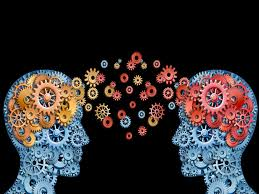
\includegraphics[scale=0.50]{figures/prework}
                            \newline
                            {\tiny Tomado de la referencia [1] }
                            \caption{ Trabajo previo. }
                        \end{figure}
            
                    \item Ofrecer nuevas ideas, perspectivas y enfoques.
                        \begin{figure}
                            
\includegraphics[scale=0.15]{figures/newIdeas}
                            \newline
                            {\tiny Tomado de la referencia [2] }
                            \caption{Nuevas ideas.}
                        \end{figure}
                        \asuivre
                \end{enumerate}
            \end{multicols}
    \end{frame}


    \begin{frame}
        \frametitle{Comprender el papel de la revisi\'on de la literatura} 
        \begin{multicols}{2}
            \begin{enumerate}
                \suite
                \item Posibles personas para recibir asesoramiento.
                \begin{figure}
                    
\includegraphics[scale=0.10]{figures/asesoramiento}
                    \newline
                    {\tiny Tomado de la referencia [3] }
                    \caption{ Asesoramiento. }
                \end{figure}

                \item Metodolog\'ia de trabajo de otros.
                \item Fuentes de datos que no conoc\'ia.
                    \begin{figure}
                        
\includegraphics[scale=0.40]{figures/newResources}
                        \newline
                        {\tiny Tomado de la referencia [4] }
                        \caption{Nuevas referencias.}
                    \end{figure}
                    \asuivre
            \end{enumerate}
        \end{multicols}
    \end{frame}

     \begin{frame}
        \frametitle{Comprender el papel de la revisi\'on de la literatura} 
        \begin{multicols}{2}
            \begin{enumerate}
                \suite
                \item Herramientas de medici\'on de otros investigadores.
                \begin{figure}
                    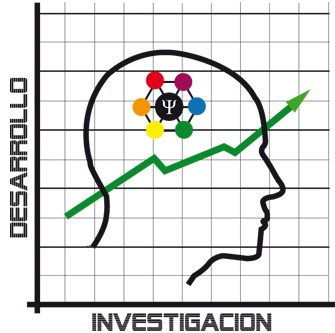
\includegraphics[scale=0.40]{figures/medicion}
                    \newline
                    {\tiny Tomado de la referencia [5] }
                    \caption{Gr\'aficos de resultados. }
                \end{figure}

                \item M\'etodos para lidiar con dificultades.
                \item Interpretar y dar sentido a los resultados.
                    \begin{figure}
                        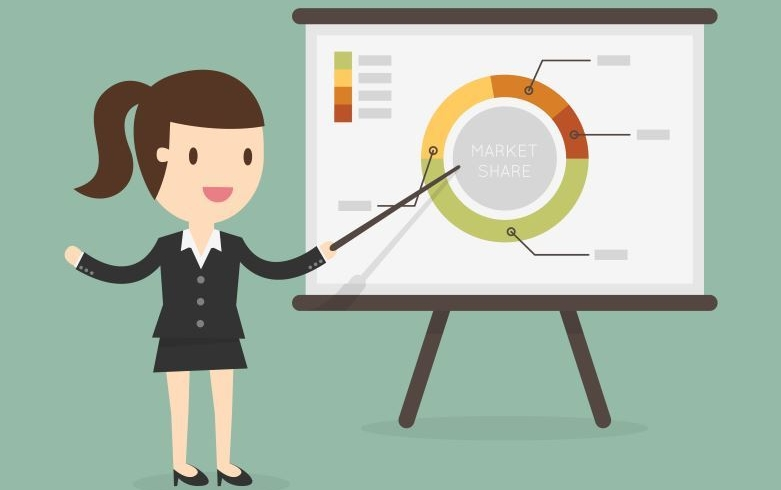
\includegraphics[scale=0.60]{figures/resultsOriented}
                        \newline
                        {\tiny Tomado de la referencia [6] }
                        \caption{Entender resultados.}
                    \end{figure}
                    \asuivre
            \end{enumerate}
        \end{multicols}
    \end{frame}

     \begin{frame}
        \frametitle{Comprender el papel de la revisi\'on de la literatura} 
            \begin{enumerate}
                \suite
                \item Reforzar la confianza en que vale la pena estudiar su tema.
                \begin{multicols}{2}
                    \begin{figure}
                        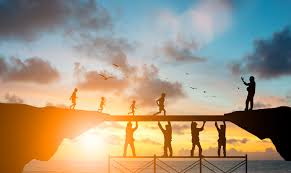
\includegraphics[scale=0.50]{figures/confianza}
                        \newline
                        {\tiny Tomado de la referencia [7] }
                        \caption{ Confianza. }
                    \end{figure}

                    \begin{figure}
                        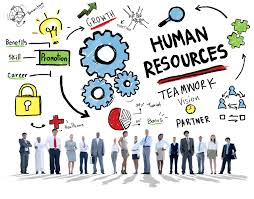
\includegraphics[scale=0.50]{figures/recursos}
                        \newline
                        {\tiny Tomado de la referencia [8] }
                        \caption{ Recursos invertidos. }
                    \end{figure}
                \end{multicols}
            \end{enumerate}       
    \end{frame}

\section{Localizar literatura relacionada} 
    \begin{frame}
    \frametitle{Estrategias para localizar literatura relacionada}
        \begin{multicols}{2}            
            \begin{itemize}
                \item Muchos recursos disponibles.  
                \item Enfocar la b\'usqueda. 
                \item \textbf{Palabras clave.} 
                \item Use libros y publicaciones con fechas de copyright recientes.                    
            \end{itemize}                 
            \begin{figure}
                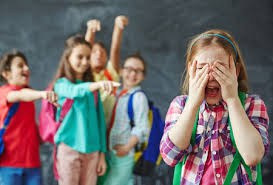
\includegraphics[scale=0.60]{figures/bullying}
                \newline
                {\tiny Tomado de la referencia [9] }
                \caption{ Ejemplo de Bullying. }
            \end{figure}                    
        \end{multicols}
    \end{frame}

    \subsection{Cat\'alogo de la biblioteca}
        \begin{frame}\frametitle{Cat\'alogo de la biblioteca}
            \begin{itemize}
                \item Publicaciones peri\'odicas que posee la biblioteca.                
                \item Sistema de clasificaci\'on Dewey Decimal (DD).
                \item Sistema de clasificaci\'on de la Biblioteca del Congreso (LC).                 
            \end{itemize} 
            \begin{figure}
                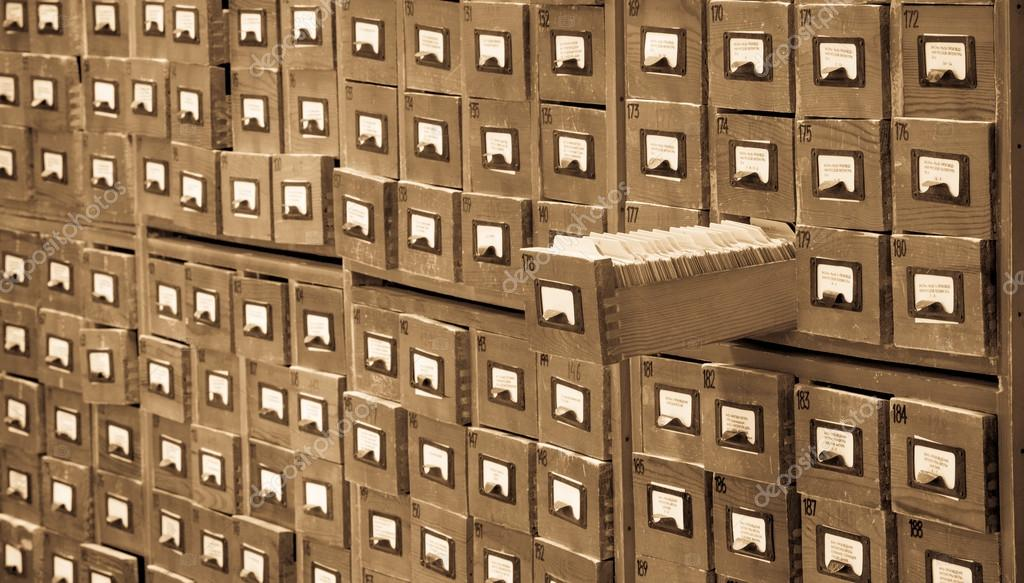
\includegraphics[scale=0.15]{figures/catalogoBiblioteca}
                \newline
                {\tiny Tomado de la referencia [10] }
                \caption{ Cat\'alogo. }
            \end{figure}      
        \end{frame}

    \subsection{\'Indices and Abstracts}
    \begin{frame}
    \frametitle{\'Indices and Abstracts}
        \begin{multicols}{2}  
            \begin{itemize}
                \item \textbf{\'Indice: } Incluye art\'iculos, informes de investigaci\'on y otros documentos. 
            \end{itemize}
            \begin{itemize}
                \item \textbf{Abstract: } Proporciona la fuente del estudio original. 
            \end{itemize}  
        \end{multicols}
        \begin{figure}
            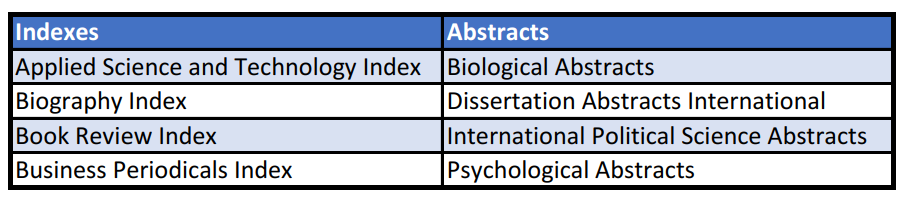
\includegraphics[scale=0.45]{figures/index}       
        \end{figure}  
    \end{frame}

    \subsection{Bases de datos en l\'inea}
        \begin{frame}\frametitle{Bases de datos en l\'inea}
            \begin{itemize}
                \item Permiten b\'usquedas en miles de revistas y otras fuentes.  
                \item Ubicar fuentes de informaci\'on disponibles en la biblioteca.
            \end{itemize} 
            \begin{figure}
                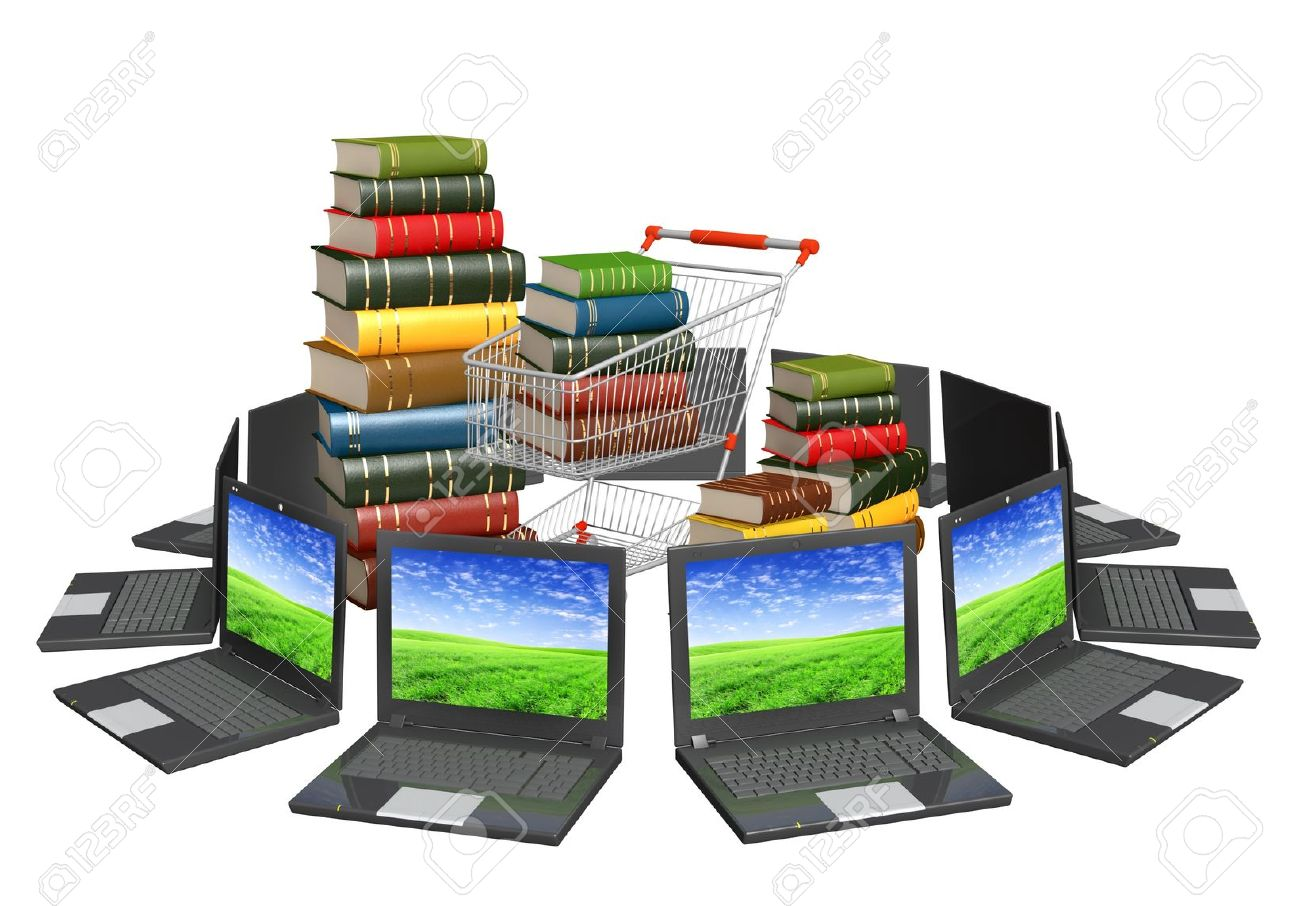
\includegraphics[scale=0.45]{figures/onlineDB}
                \newline
                {\tiny Tomado de la referencia [11] }
                \caption{ Base de datos en l\'inea. }
            \end{figure} 
        \end{frame}

    \subsection{Bibliotecarios de referencia}
    \begin{frame}\frametitle{Bibliotecarios de referencia}
        \begin{multicols}{2}  
            \begin{itemize}
                \item Demostrar c\'omo usar los recursos. 
                \item La mejor manera de dominar la biblioteca es usarla.  
            \end{itemize} 
             \begin{figure}
                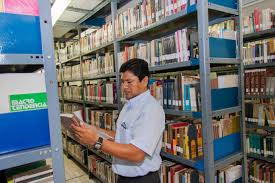
\includegraphics[scale=0.45]{figures/bibliotecario}
                \newline
                {\tiny Tomado de la referencia [12] }
                \caption{Bibliotecario. }
            \end{figure}
        \end{multicols}       
    \end{frame}

    \subsection{Navegar por Internet}
    \begin{frame}\frametitle{Navegar por Internet}
    \begin{multicols}{2}  
        \begin{itemize}
            \item Indicaciones importantes. 
                \begin{enumerate}
                    \item Usar al menos dos palabras clave.
                    \item Escriba un signo m\'as (+) antes de cualquier palabra clave.
                    \item Ponga comillas alrededor de la frase.
                \end{enumerate} 
            \item Siempre que encuentre informaci\'on, debe anotar el URL y la fecha.
        \end{itemize} 
        \begin{figure}
                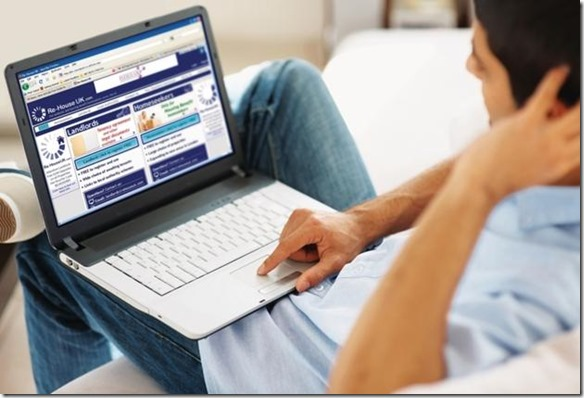
\includegraphics[scale=0.25]{figures/navWeb}
                \newline
                {\tiny Tomado de la referencia [13] }
                \caption{Navegar por internet. }
            \end{figure}
        \end{multicols}
    \end{frame}

   \begin{frame}
   \frametitle{Uso de citas y listas de referencias de los que se han ido antes}
        \begin{itemize}
            \item Valiosa orientaci\'on sobre estudios de investigaci\'on.  
            \item Rastrear cualquier referencia que vea citada por tres o m\'as investigadores.
            \item \textbf{Siempre que sea posible, vaya a la fuente original y l\'eala usted mismo.}
        \end{itemize} 
    \end{frame}

\section{B\'usqueda de literatura} 
 \begin{frame}\frametitle{B\'usqueda de literatura}
    \begin{multicols}{2}  
        \begin{itemize}
            \item Seleccionar un problema o pregunta de investigaci\'on.
            \item Enfoque de \emph{\enquote{Divide y vencer\'as}}.
        \end{itemize} 
        \begin{figure}
                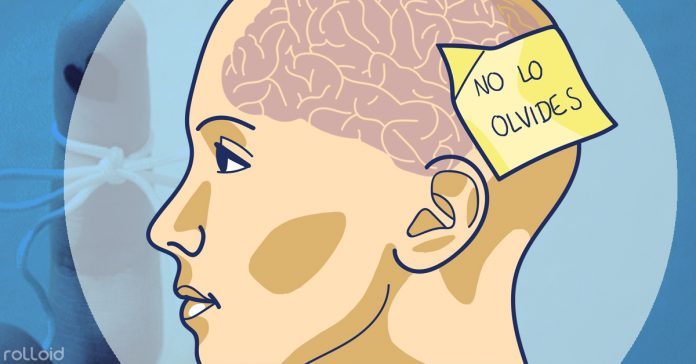
\includegraphics[scale=0.25]{figures/recordar}
                \newline
                {\tiny Tomado de la referencia [14] }
                \caption{Importante de recordar. }
            \end{figure}
        \end{multicols}
    \end{frame}

    \subsection{Utilizar el tiempo de biblioteca de manera eficiente}
        \begin{frame}\frametitle{Usar su tiempo de biblioteca de manera eficiente}
        \begin{multicols}{2}
            \begin{enumerate}
                \item Disponer de herramientas de recopilaci\'on de datos.
                \item Identificar el material y la disponibilidad.
                \item Desarrollar un plan de ataque. 
                \item Busque sus fuentes.            
                \asuivre
            \end{enumerate}
             \begin{figure}
                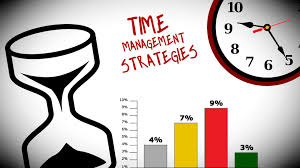
\includegraphics[scale=0.45]{figures/timeManagement}
                \newline
                {\tiny Tomado de la referencia [15] }
                \caption{Manejo del tiempo. }
            \end{figure}
        \end{multicols}
        \end{frame}
        \begin{frame}\frametitle{Usar su tiempo de biblioteca de manera eficiente}
        \begin{multicols}{2}
            \begin{enumerate}
                \suite
                \item Registre toda la informaci\'on b\'asica mientras lee cada fuente.
                \item Identifique estrategias para obtener fuentes que no est\'an disponibles.            
                \asuivre
            \end{enumerate}
             \begin{figure}
                
\includegraphics[scale=0.20]{figures/timeManagement2}
                \newline
                {\tiny Tomado de la referencia [16] }
                \caption{Manejo de los recursos. }
            \end{figure}
        \end{multicols}
         \end{frame}

    \subsection{Evaluar la investigaci\'on de otros}
        \begin{frame}
        \frametitle{Evaluar la investigaci\'on de otros}
        \begin{multicols}{2}
            \begin{enumerate}
                \item Determinar ideas, hallazgos de investigaci\'on y conclusiones.
                \item Conciliar los hallazgos inconsistentes obtenidos.
                \item Ideas sobre c\'omo puede mejorar sus propios esfuerzos.        
                \asuivre
            \end{enumerate}
             \begin{figure}
                
\includegraphics[scale=0.45]{figures/checklist}
                \newline
                {\tiny Tomado de la referencia [17] }
                \caption{Evaluar. }
            \end{figure}
        \end{multicols}
        \end{frame}

\section{Escribir la rese\~na de la literatura}
    \begin{frame}\frametitle{Escribir la rese\~na de la literatura}
    \begin{multicols}{2}
                \begin{enumerate}                    
                    \item Obtener la orientaci\'on psicol\'ogica adecuada.
                    \item Tener un plan.  
                    \item Enfatizar la relaci\'on con su problema de investigaci\'on.         
                    \asuivre
                \end{enumerate}
                \begin{figure}
                    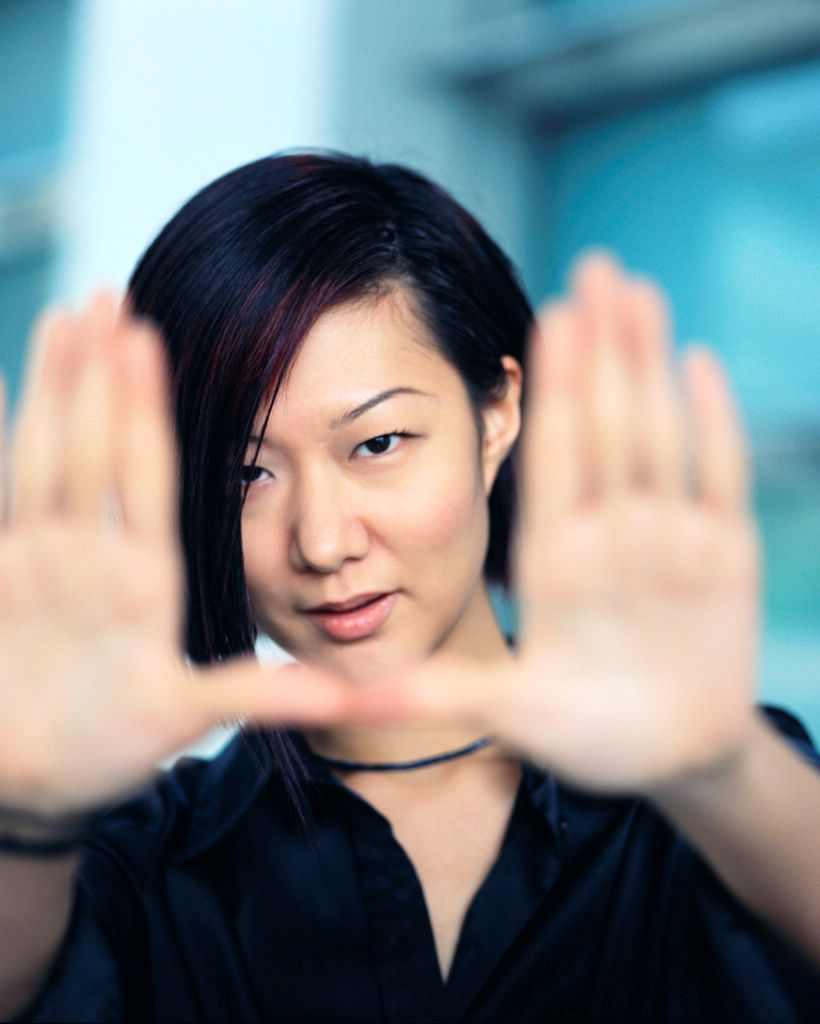
\includegraphics[scale=0.10]{figures/focus}
                    \newline
                    {\tiny Tomado de la referencia [18] }
                    \caption{Manejo de los recursos. }
                \end{figure}
            \end{multicols}
    \end{frame}

    \begin{frame}\frametitle{Escribir la rese\~na de la literatura}
    \begin{multicols}{2}
                \begin{enumerate}
                    \suite
                    \item Utilizar frases de transici\'on.
                    \item Diferenciar entre escribir la literatura y plagiarla.  
                    \item Siempre dar cr\'edito.       
                    \item Minimice el uso de citas directas del trabajo de otras personas.    
                    \asuivre
                \end{enumerate}   
                \begin{figure}
                    \includegraphics[scale=0.30]{figures/plagio}
                    \newline
                    {\tiny Tomado de la referencia [20] }
                    \caption{Plagio. }
                \end{figure}               
            \end{multicols}
    \end{frame}

    \begin{frame}\frametitle{Escribir la rese\~na de la literatura}
    \begin{multicols}{2}
                \begin{enumerate}
                    \suite
                    \item Resuma lo que dijo.
                    \item Recuerde que su primer borrador seguramente no ser\'a el \'ultimo. 
                    \item Pida consejos y comentarios a los dem\'as.                   
                \end{enumerate}         
                \begin{figure}
                    \includegraphics[scale=0.45]{figures/borrador}
                    \newline
                    {\tiny Tomado de la referencia [19] }
                    \caption{Borradores. }
                \end{figure}      
            \end{multicols}
    \end{frame}

\section{Conclusiones}
    \begin{frame}\frametitle{Conclusiones}
        \begin{enumerate}                    
            \item Seleccione un tema que sea de su inter\'es.
            \item Haga un trabajo de investigaci\'on previa antes de comenzar a trabajar. 
            \item Recuerde que hacer una buena revisi\'on de la literatura puede ahorrarle mucho tiempo y trabajo.                   
        \end{enumerate}   
    \end{frame}

    \begin{frame}%%     2
    \begin{center}
    {\fontsize{25}{30}\selectfont Muchas gracias.}
    \end{center}
    \end{frame}

\begin{frame}\frametitle{Referencias}
    \begin{thebibliography}{1}
        \bibitem{[1]} Harmonia (2011) \emph{Beneficios de compartir con los demas} [Blog post]. Consultado desde https://harmonia.la/comunidad/3\_beneficios\_de\_compartir\_tu\_conocimiento\_con\_los\_demas
        \bibitem{[2]} \emph{Grandes ideas} (2012). Consultado desde https://cbncuritiba.com/sua-carreira-em-pauta-empresa-junior-pode-ser-ponto-de-partida-para-experiencia-profissional/empresario-com-uma-grande-ideia\_1012-219/ 
        \bibitem{[3]} \emph{Asesoramiento profesional.}. Consultado desde http://www.gorbeialdea.com/es/turismo/profesionales/competitividad/asesoramiento-empresarial.html
        \bibitem{[4]} \emph{Asombro.} (2001). Consultado desde https://definicion.de/asombro/   
    \end{thebibliography}
    \end{frame}

\begin{frame}\frametitle{Referencias}
    \begin{thebibliography}{1}
        \bibitem{[5]}Fundamentos de psicologia educativa. \emph{Instrumentos de medici\'on.} Consultado desde http://fundamentosdepsicologiaeducativa.blogspot.com/2017/05/41-concepto-de-medicion-42-instrumentos.html
        \bibitem{[6]} \emph{Interpretaci\'on de los resultados.}. Consultado desde http://lesbos.webcam/camwhores/interpretacion-de-los-resultados-de.html
        \bibitem{[7]} \emph{Bullying.}. Consultado desde http://www.gorbeialdea.com/es/turismo/profesionales/competitividad/asesoramiento-empresarial.html
   \end{thebibliography}
    \end{frame}

\begin{frame}\frametitle{Referencias}
    \begin{thebibliography}{1}
        \bibitem{[9]} UDEP  (2013) \emph{Celebran d\'ia del bibliotecario.} Consultado desde http://udep.edu.pe/hoy/2013/celebraran-el-dia-del-bibliotecario/
        \bibitem{[10]} \emph{Recordar.} (2018). Consultado desde https://rolloid.net/recordar-practicamente-cualquier-cosa-utilizando-metodo-loci/
        \bibitem{[11]} \emph{Meritocracia}. Consultado desde https://www.youtube.com/watch?v=SHiSe6-mOiY
        \bibitem{[12]} \emph{Manejo del tiempo.}  Consultado desdehttps://www.businessforunicorns.com/time-management-two-things/    
    \end{thebibliography}
    \end{frame}

\begin{frame}\frametitle{Referencias}
    \begin{thebibliography}{1}
        \bibitem{[13]} \emph{Asesoramiento}. Consultado desde https://blog.aritraroy.in/the-ultimate-pre-release-checklist-for-android-app-success-on-play-store-cb0eb9f59ce9?gi=4e2377dd4dd1
        \bibitem{[14]} \emph{Traffic jam.}. Consultado desde http://www.thedrive.com/accelerator/602/the-10-biggest-traffic-jams-ever
        \bibitem{[15]} \emph{Borradores.} (2012). Consultado desde https://draft.com/
        \bibitem{[16]} \emph{Latex-Tutorial.} (2018). Consultado desde https://www.latex-tutorial.com        
    \end{thebibliography}
    \end{frame}
\begin{frame}\frametitle{Referencias}
    \begin{thebibliography}{1}
        \bibitem{[17]}The Editors of Encyclopaedia Britannica  (2013) \emph{LaTeX COMPUTER PROGRAMMING LANGUAGE} [Blog post]. Consultado desde https://www.britannica.com/technology/LaTeX-computer-programming-language
        \bibitem{[18]} \emph{Introduction to LaTeX.} (2018). Consultado desde https://www.latex-project.org/about/
        \bibitem{[19]} \emph{Checklist image.} (1994). Consultado desde https://blog.aritraroy.in/the-ultimate-pre-release-checklist-for-android-app-success-on-play-store-cb0eb9f59ce9?gi=4e2377dd4dd1
          
    \end{thebibliography}
    \end{frame}

    \begin{frame}\frametitle{Referencias}
    \begin{thebibliography}{1}
    \bibitem{[20]} \emph{Focus and You Will Succeed} (2000). Consultado desde  http://www.tameraaragon.com/focus-and-you-will-succeed/     
    \bibitem{[8]} \emph{Servidores inform\'aticos.} Consultado desde https://pt.dreamstime.com/foto-de-stock-conceito-da-tecnologia-de-armazenamento-do-servidor-de-informa%C3%A7%C3%A3o-do-base-de-dados-image77457469    
    \end{thebibliography}
    \end{frame}
\end{document}